\section{Magnitude Estimation and Crowdsourcing}
\label{sec:cs}

We now turn to the second research question RQ\ref{item:rq4} and 
investigate whether crowdsourcing is a valid methodology to gather magnitude
estimation scores. 
We have already touched upon several related issues: the quality
checks that we put in place in our experiment and that allowed us to
gather good quality data (Section~\ref{sec:quality-checks}); the
approximately log-normal distribution of our magnitude estimation
scores (Section~\ref{sec:score-distribution}); the normalization and
aggregation functions (Section~\ref{sec:score-normalization}); and the
overall agreement of the magnitude estimation scores with official
relevance judgments (Section~\ref{sec-rq1}). 
We now present more details, focusing on measuring judge
agreement, on analyzing disagreement with official judges, and on
discussing what happens when the number of collected judgments 
decreases.

%\fs{ We didn't record the ``rubbish'' workers, they were prevented
%  from carrying out the task, so we can't do an analysis of what
%  happens if they are kept in.
%  Let's keep this RQ for later in the paper, and in that place repeat
%  some of the analysis using the median of 5 and 3 (instaed of 10) ME
%  judgments?}
%
%\sm{I've left this note here but I'm not sure I understand it...}

\subsection{Judge Agreement and Quality}
 \label{sec:judge-agreement}
It is well-known that relevance is subjective, even when focusing on
``topical'' relevance as is typically done in evaluation campaigns such
as TREC, and that judges will therefore not perfectly agree.
We define and discuss two kinds of agreement:
\begin{itemize}
\item \emph{internal}: agreement within one group of workers judging the
  same topic-document pair; and 
\item \emph{external}: agreement with expert judges (TREC,
  Sormunen). 
\end{itemize}
  
\subsubsection{Internal Agreement}
\label{sec:internal-agreement}

In our data, there are
at least ten workers judging the same topic-document pair, and
the source of internal disagreement might be threefold:
(i) the arbitrary, personal scale used by a judge when expressing an ME
score; 
(ii) the subjective nature of relevance; and 
(iii) the often-feared low quality of work in crowdsourcing exercises.
The first has already been discussed and is removed by the geometric
average normalization process (Section~\ref{sec:score-normalization}).
The second is a feature that one might not want to remove from the
data: different judges can truly have different opinions on the
relevance of a document, whatever scale of measurement is used.
Usually IR evaluators assume that this variation is distilled into a single 
value (for example: mean, median or mode) 
that represents a population of users \textcolor{red}{(although there might in fact not be a unique truth~\citep{aroyo2015truth})}.
Of course, the third source is in need of particular attention: low
quality workers might express unreliable scores, and in general this
would lead to low internal agreement.

To examine internal agreement, we can investigate the spread of 
the 10 normalized scores collected for each topic-document pair.
Being on a ratio scale, an appropriate way of quantifying the upper
limit of the spread is
by the ratio between maximum and minimum $\max(s'_i) / \min(s'_i)$.  
Figure~\ref{fig:judgeVariability} 
shows the distribution of the ratio in our data.
Another measure of dispersion that can be used is the geometric
standard deviation (a version of standard deviation adapted for
geometric mean and log-normal distributions). 
The chart on the right of the figure shows that the geometric standard
deviation correlates quite well with the max/min ratio (Pearson's
correlation is $0.999$), and therefore is an almost equivalent
measure. 

\begin{figure}[tp]
  \centering
  \includegraphics[width=.9\linewidth,page=6]{figs/JudgeVariability.pdf}
%  \includegraphics[width=.29\linewidth,page=2]{figs/MaxMin-gsd_corr.pdf}
  \caption{Number of documents with a $\max(s_i) / \min(s_i)$ ratio in
    a particular range (rounded to the nearest 5), out of 4269 documents.  
    The inner panel shows a scatterplot of the correlation
    between
    $\max(s_i) / \min(s_i)$ ratio and the geometric standard deviation
    (log scale;  the blue dots on the bottom are
    the 34 out of the 36 \nkn and \hkh documents, which received many
    more judgments and therefore exhibit a higher ratio; 7 points are
    left out, including the two missing  \nkn / \hkh documents). 
    \label{fig:judgeVariability}
  }
\end{figure}

While it is difficult to make conclusions about the absolute values of
the ratio or geometric standard deviation without some reference point, it does highlight, for
example, that there are 23 documents that seem to have an
unusually high ratio of 10000 or more.
Looking at each of these cases, there are two distinct causes.
Firstly, 15 of the 23 looked like genuine attempts to assign ME scores,
but the range of scores for each worker involved was very wide.
One reason given in the comments by workers was that there was no zero
available, so for documents that were truly off topic, they chose an
arbitrary, very very small, number, making a wide scale.
These wide scales were not markedly compressed by the normalization
stage.
In some cases the numbers assigned seemed arbitrary, but suitably
large or small in correlation with the expert judgments.
The second cause, in 8 of the 23 cases, seemed to be workers not
following instructions or reading documents carefully.
In these cases the comments provided by the workers bore no
relationship to their numeric scores, and the numbers themselves
seemed arbitrary.
We will discuss the seemingly arbitrary nature of some scores later on
(Section~\ref{sec:sig-figs}). 

Another way of examining internal (intra-assessor) agreement is through
measures of reliability. Krippendorff's $\alpha$ \citep{HayKri07} is a
widely-used reliability measure that is defined for different types of
measurement scales.
$\alpha$ is a chance-corrected measure
of reliability, taking into account both observed and expected
agreement.
For ratio-level data, the $\alpha$ difference function is defined as
square of the ratio of the difference between a pair of values assigned
by two judges to
the sum of the values assigned by the same pair of judges \citep{Kri11}.

Across the full set of 4,269 topic-document pairs, $\alpha=0.323$
(recall that each item received at least 10 independent judgments; for
the few items where a larger number of judgments were collected, the
first 10 responses are used).
Based on a bootstrap hypothesis test, this level of agreement is
significantly different from zero agreement ($p<0.01$).
We note that the numeric value of $\alpha$ is difficult to interpret in
this context, as to the best of our knowledge this is the first
investigation of document-level relevance judgments using magnitude
estimation, so no direct comparison is available.

Overall, the data show a not perfect but reasonably high
internal agreement.

\subsubsection{External Agreement and Quality of Workers}
\label{sec:external-agreement}

We now turn to analyze the external agreement, namely the agreement
with the ``official'' TREC and Sormunen judges. 
In passing we also investigate the level of agreement when using
different scales for judging relevance. 
We have already discussed the overall consistency with the official
judges in Section~\ref{sec-rq1}. 
%Section~\ref{sec:cons-magn-estim}. 
Here the results of a more specific analysis are shown: comparing the
pairwise orderings between binary, ordinal and magnitude estimation
relevance judgments.
For example, 
if two documents are rated \nn and \mm on the ordinal scale, 
and the corresponding
magnitude estimation score of the first is lower than or equal to the
score for the second, this would be counted as an agreement.
If the
magnitude estimation score was higher for the second document, it
would indicate disagreement.
Intuitively, we can estimate that a worker has a high quality if the
number of pairs of documents are ordered as in TREC or Sormunen.
This measure of the quality of our crowdsourcing workers is reasonable
even if the scales of the judgments differ, as long as they impose a
ranking on the documents. 

\begin{figure}[tp]
  \centering
  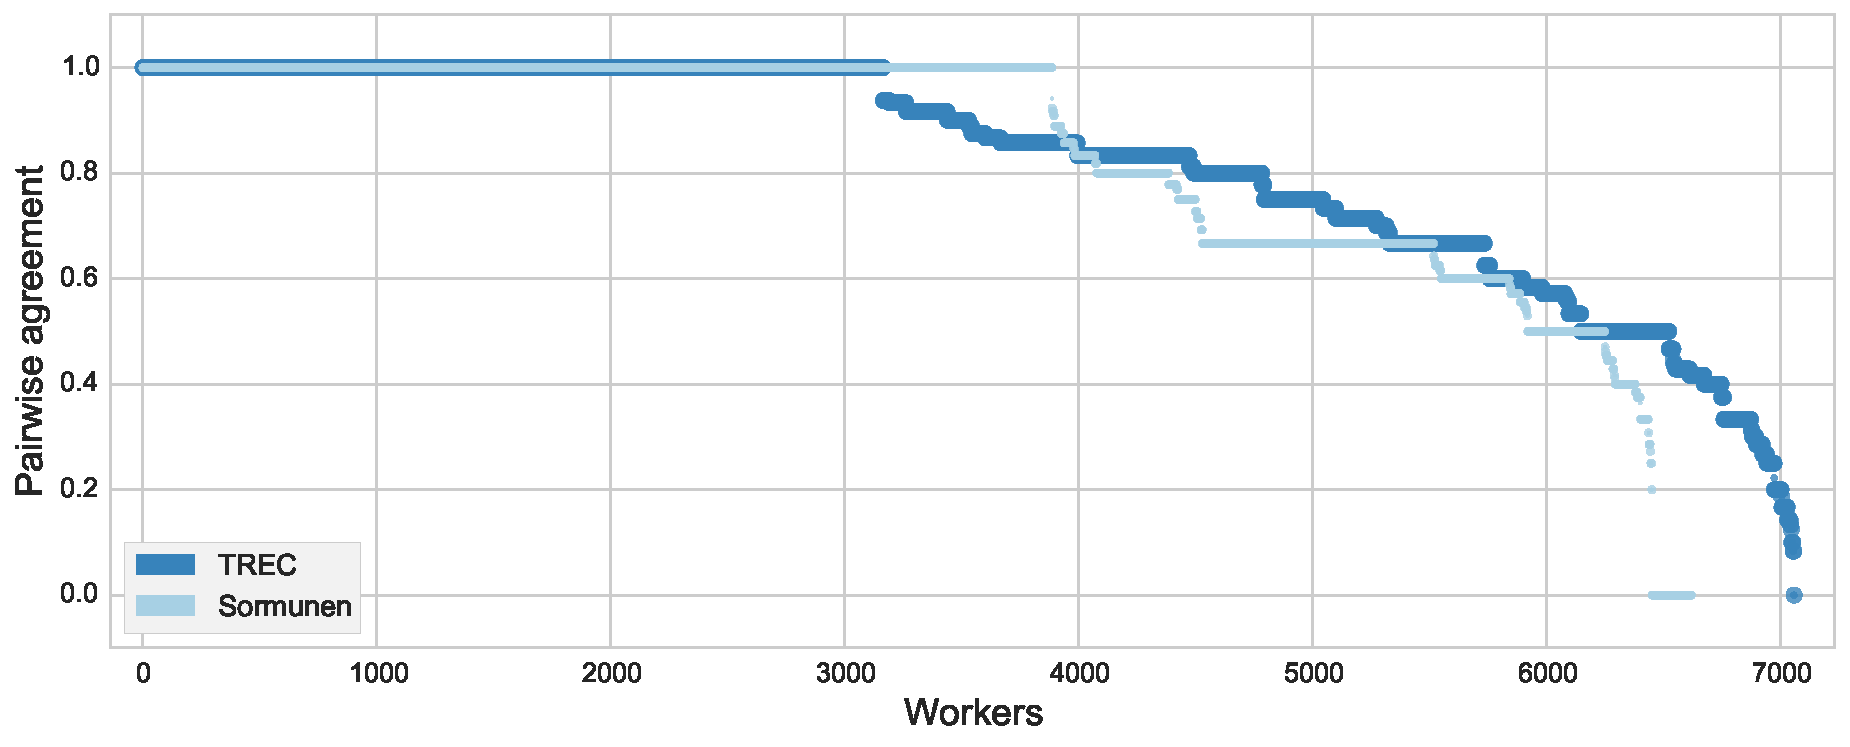
\includegraphics[width=.9\linewidth]{figs/WorkersQuality.pdf}
  \caption{Agreement over the ranking of all pairs of documents for individual units 
    using worker-assigned ME scores versus
    TREC or Sormunen categories. The number of pairs for each
    unit may vary, since some of the documents might be unjudged on the ordinal scales.
    % \fs{Need to remove the graph ``title'' in this and subsequent new
    % graphs. Also the y-axis could usefully be more informative than
    % ``quality'', e.g. ``Pairwise agreement''}
    % \aht{Also, use ``Sormunen'' and ``TREC'' in the legend. This graph might be better reverse
    %      sorted, so we can easily read off that 3000/4000 workers agree 100\%.}
    \label{fig:workersQuality}}
\end{figure}


Figure~\ref{fig:workersQuality} shows, for each unit, the pairwise
agreement with both TREC and Sormunen judgments. 
Workers are generally good using this metric, with 
around 50\% of the workers having perfect agreement; 
around 70\% an agreement higher than $0.8$; and 
around 86\% of the workers have an agreement higher than $0.6$.
Note that as there are many documents unjudged on the Sormunen
scale, thus 2376 units have only one pair of 
documents on which to compute agreement, contributing 
to the appearance 
of workers agreeing more with Sormunen than TREC using this metric.



\begin{figure}[tp]
  \centering
  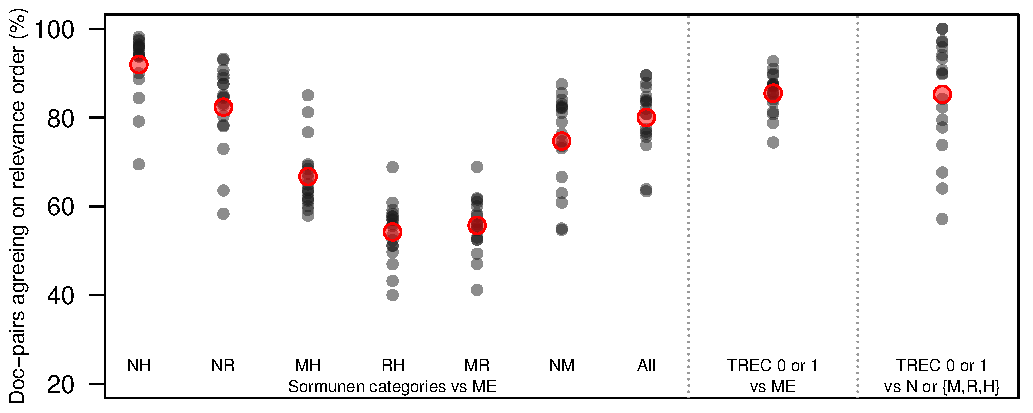
\includegraphics[width=.75\linewidth]{figs/pairwise5.pdf}
  \vspace{-0.0cm}
  \caption{Raw agreement on the ordering of relevance of all document pairs (one
small dot per topic) between judges as indicated on the x-axis (ME: magnitude
estimation). The large (red) dot is the mean over all topics in each case. 
    Unjudged documents are excluded.
  \label{fig:agreement}
}
\end{figure}

% From AHT:
% Figure 7
% 
% Mean   NH:     91.939%
% Mean   NR:     82.340%
% Mean   MH:     66.704%
% Mean   RH:     54.222%
% Mean   MR:     55.693%
% Mean   NM:     74.701%
% Mean  All:     80.027%
% Mean TvsME:    85.499%
% Mean TvsS:     85.237%


Figure~\ref{fig:agreement} shows the agreement data stratified by each of the possible six pairs of
ordinal relevance levels of the Sormunen judgments (first six columns)
and ungrouped (seventh column).
The TREC vs.\ ME comparison, aggregated over all topics, is shown in the
eighth column, and for comparison, the final column shows the pairwise
agreement between TREC and Sormunen, assuming that 
\nn equates  to TREC category ``0'', and the other three Sormunen categories 
equate to TREC category ''1''.
Red large circles indicate the mean score over the 18 topics for each group.
It can be seen that the rates of agreement are highly consistent when
comparing any of the three relevance scales.
In particular, ME scores for \hh documents are greater than those for 
\nn documents 92\% of the time (mean, first column), which is
higher than the average agreement between TREC and Sormunen
(85\%---mean, last column).
Similarly, the proportion of document pairs that have different TREC
categories are ranked in the same order by ME scores 86\% of the time
(mean, second last column).
%The agreement between 
ME  and Sormunen ranking for documents in the \nn\rr category
also agree 82\% of the time (mean, second column), and over all pairs
Sormunen and ME agree 80\% of the time (mean, seventh column).
This overall average is reduced by the lower agreements between pairs
of documents that are deemed relevant and one or other are in the 
\mm or \rr categories (columns three to six).
This is perhaps unsurprising, as distinguishing ``marginal relevance'' (\mm)
from ``irrelevant'' (\nn) or ``relevant'' (\rr) can be difficult; and likewise 
distinguishing \rr from highly relevant (\hh) can also be challenging.

Overall, the agreement between the ME approach and the existing 
categorical judgments seem reasonable, 
further supporting the validity of the magnitude estimation
approach for gathering relevance judgments.

%%%Figure~\ref{fig:agreement} shows that there is a considerable
%%%variation over topics. 
%%%Figure~\ref{fig:workersQualityTopic} \sm{Eddy, why ``Mean'' in the
%%%  graph title??} shows a more detailed analysis:
%%%some topics have a much lower external agreement (for example, 402 and
%%%405 with Sormunen, and 421 and 427 with TREC). \sm{...}
%%%\fs{I guess that immediately raises the question of ``why??'' Again, if
%%%we want to save ``topic difficulty'' for a more robust analysis in future work,
%%%perhaps leave out this graph for now?}
%%%
%%%\begin{figure}[tp]
%%%  \centering
%%%  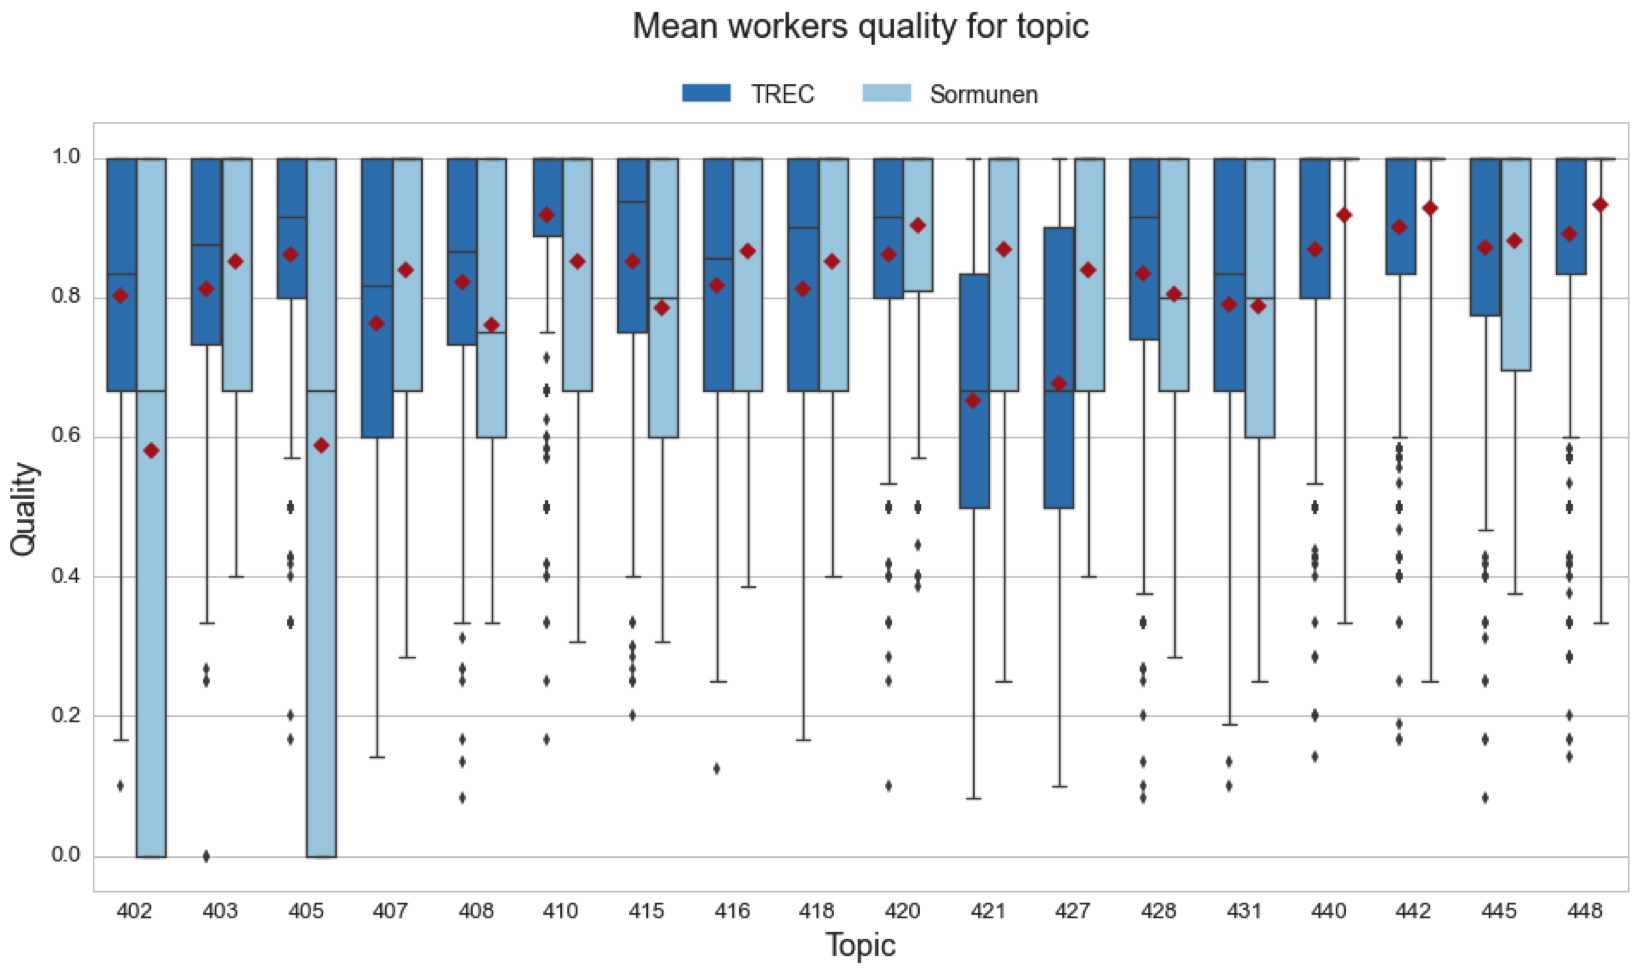
\includegraphics[width=\linewidth]{figs/WorkersQualityPerTopic.png}
%%%  \caption{Workers quality as pairwise agreement: breakdown on single topics.
%%%  \fs{Need to remove title, and change y-lab to something more precise,
%%%  such as Pairwise agreement?}
%%%  \label{fig:workersQualityTopic}}
%%%\end{figure}

\begin{figure}[tp]
  \centering
  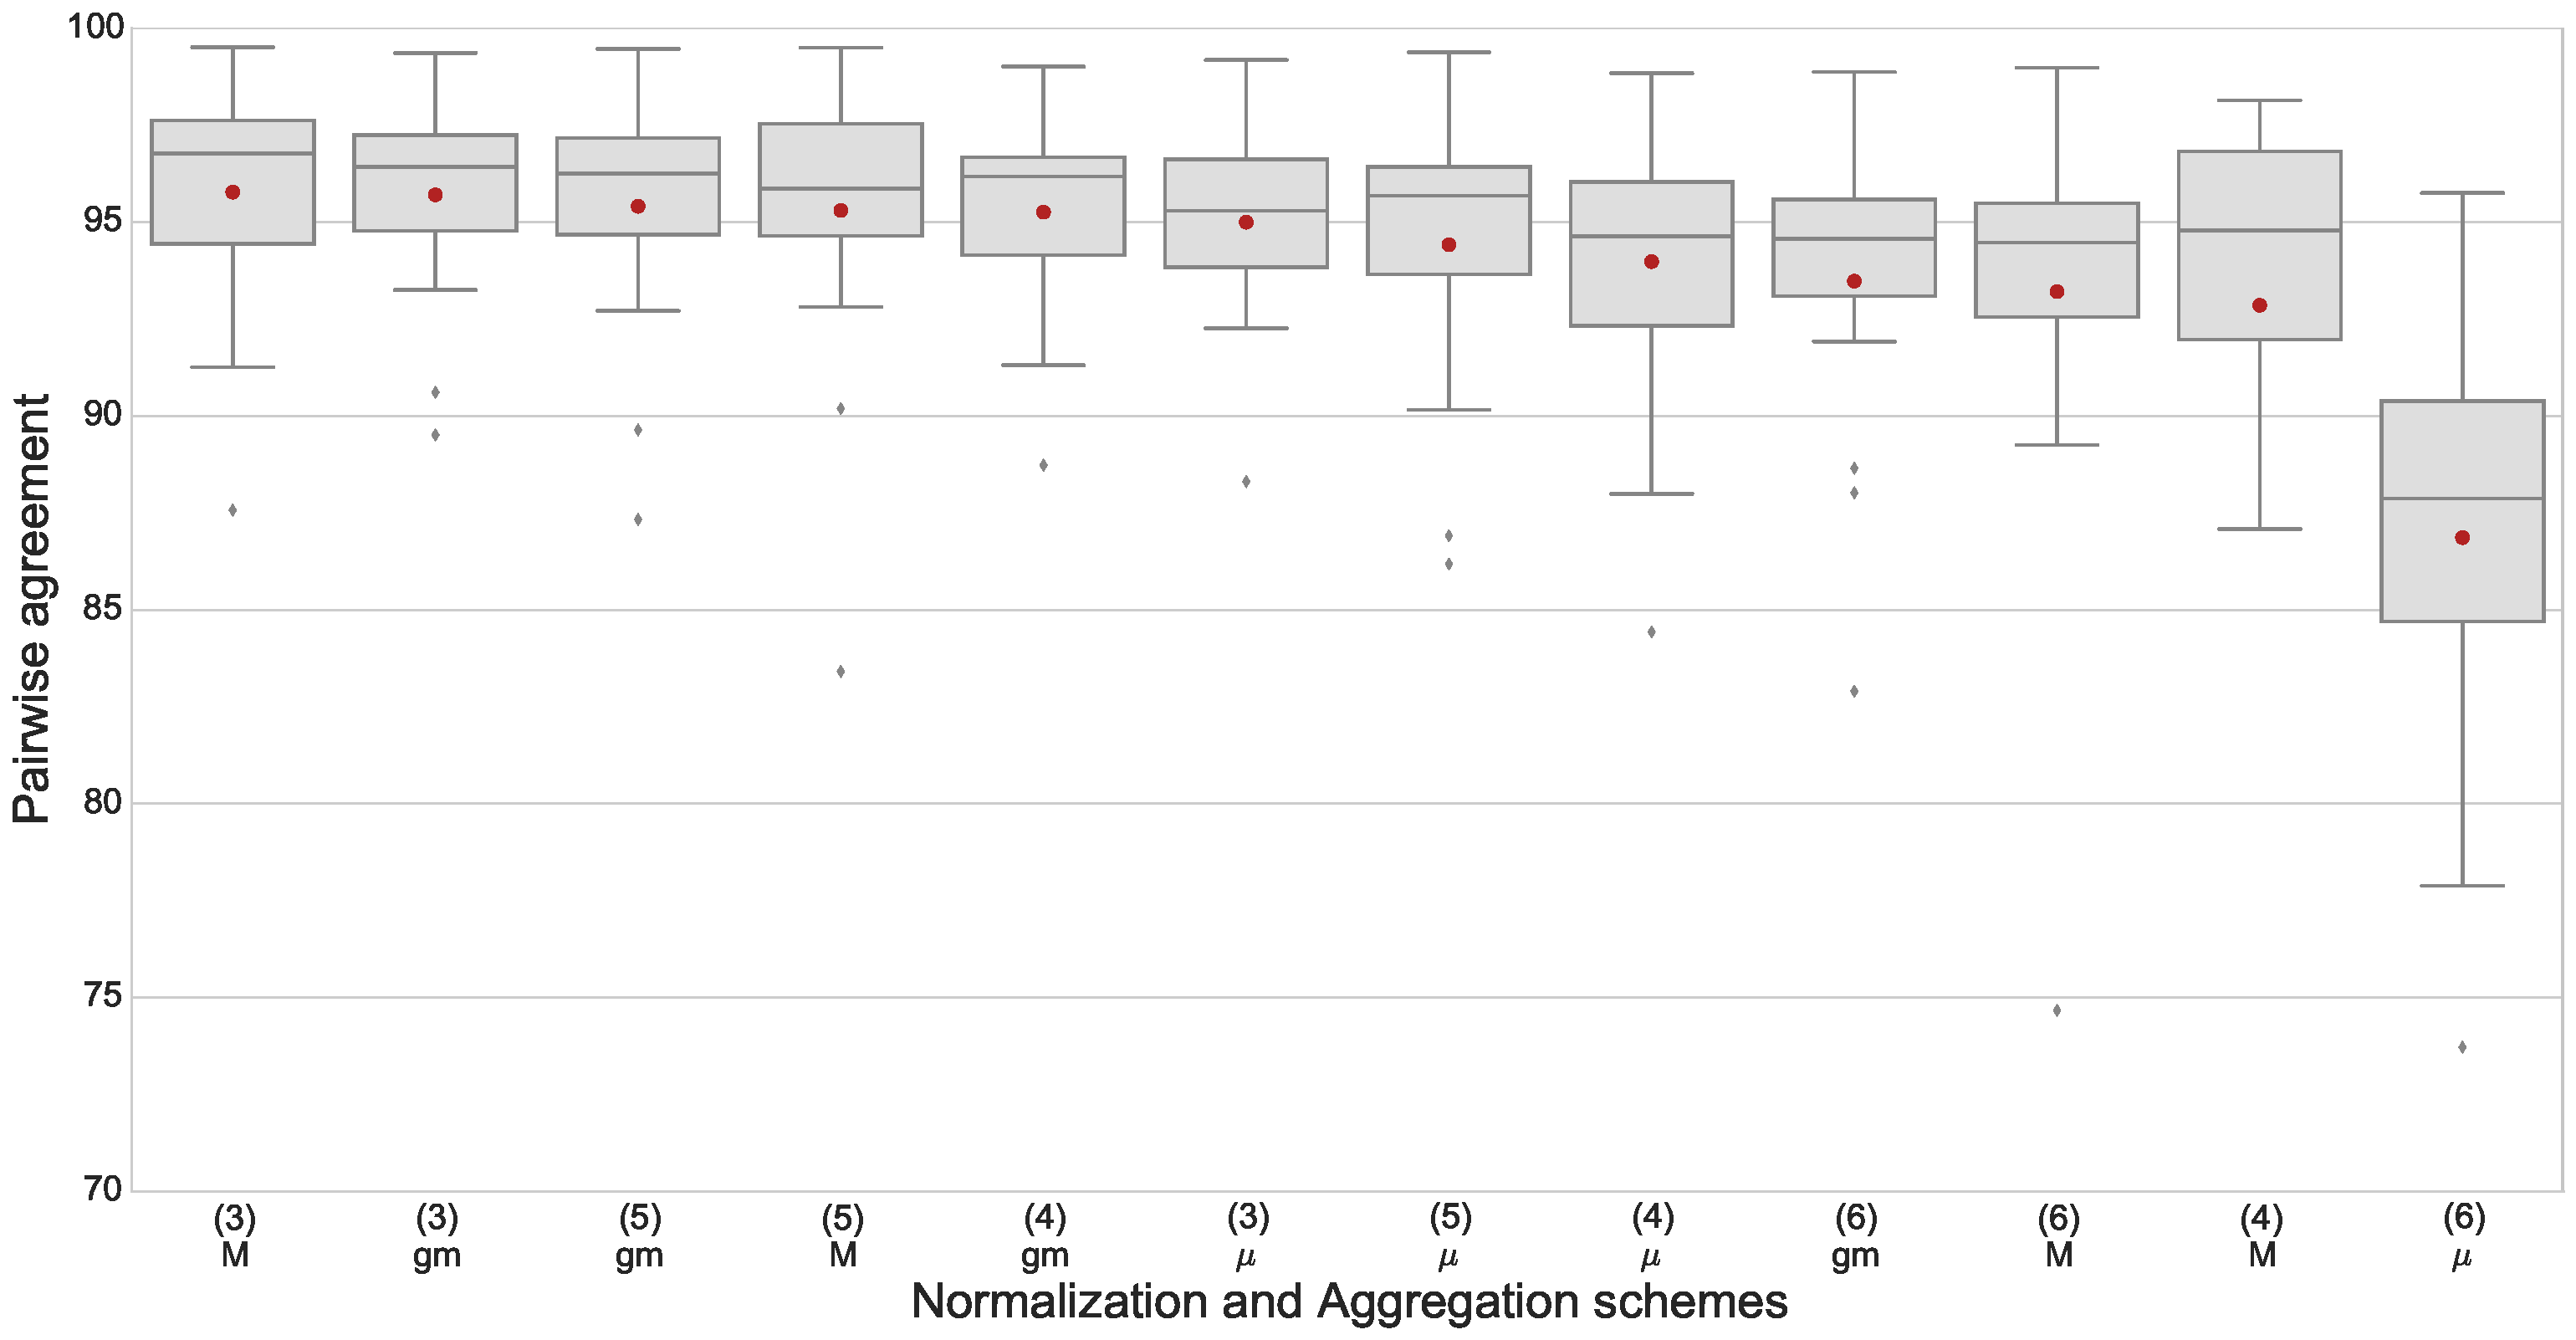
\includegraphics[width=\linewidth]{figs/aaaa/fig_box_mean.pdf}
  \caption{Effect of the four normalization functions
    (Equations~\eqref{eq:3}, \eqref{eq:4}, \eqref{eq:5}, and \eqref{eq:6}  in
    the text) and aggregation functions (\textsf{M}~=~median, \textsf{gm} = geometric mean, and
    $\mu$ = arithmetic mean) on pairwise agreement. 
%  \fs{Remove title, and change y-lab to Pairwise agreement (?)}
  \label{fig:normaggagain}}
\end{figure}


We now revisit the normalization and
aggregation issues discussed in
Section~\ref{sec:score-normalization}. We compare the following four normalization
schemas
\begin{align}
  s'_i &= e^{\log(s_i) - \mu(\log(\mathnormal{unit})) + \mu
         (\log(\mathnormal{topic})) } \label{eq:3}\\
  s'_i &= e^{\log(s_i) - M(\log(\mathnormal{unit})) +
         \mathnormal{M}(\log(\mathnormal{topic}))} \label{eq:4}\\
  s'_i &= e^{\log(s_i) - \mu (\log( \max (\mathnormal{unit})),\log(
         \min (\mathnormal{unit}))) + \mu(\log(\mathnormal{topic}))
         } \label{eq:5} \\
  s'_i &= e^{\log(s_i) - \mu(\log(\mathtt{H}_k),\log(\mathtt{N}_k)) +
         \mu (\log(\mathnormal{topic}))} \label{eq:6}
\end{align}
(where the first one corresponds to that already discussed in
Equations~\eqref{eq:1} and~\eqref{eq:2}), 
%\sm{notation is different here from Equations~\eqref{eq:1} and~\eqref{eq:2}...}  
and the three aggregation
functions mentioned at the end of
Section~\ref{sec:score-normalization}, namely median, geometric mean,
and arithmetic mean.
Figure~\ref{fig:normaggagain} shows the effect of the different
normalization and aggregation functions on the quality of the workers
measured by pairwise agreement. 
As we have discussed in Sections~\ref{sec:score-distribution}
and~\ref{sec:score-normalization}, we decided to use the somehow
standard geometric averaging (Equation~\eqref{eq:3}) plus median
normalized score. 
The chart in figure clearly shows that the selected two functions are
among those avoiding a loss of quality. 
Both when considering the medians in the boxplots and when considering
the means (the red dots in figure), on our data the highest pairwise
agreement is obtained with:
  \begin{itemize}
  \item the normalization scheme in Equation~\eqref{eq:3}, and
  \item the median or the geometric mean aggregators, rather than
    the arithmetic mean. 
  \end{itemize}

% \aht{i think we should include this, but it needs tidying up: what
%   functions did we choose and why? 
%   Do not break out by topic (fns says that is the next paper). 
%   Tidy up format of graph to look pretty. 
%   Write a bit more text (which will be easier with only one data point
%   per scheme?).}
% \sm{This is the version of the figure that I prefer: it allows to
%   discuss variety over topics/documents, if we want, but it also shows
%   clearly the order of the various combinations, and can be used to
%   justify our choice. 
%   Eddy also did some alternative versions, they are in in the folder
%   \texttt{figs/aaaa/}, have a look. 
%   Once we agree on the figure, we need to write some more organized
%   text.}
% \sm{add some more text...}
% \sm{Eddy can you re-do the figure with only the
  % ``ALL'' data: make it a barplot, maybe horizontal(?), maybe with
  % ``error bars'' representing the spread over the topics?}



\subsection{Failure Analysis}
\label{sec:failure-analysis}

Despite the similar overall levels of agreement between the magnitude
estimation method and ordinal relevance,
Figures~\ref{fig:ME-distribution}
and~\ref{fig:ME-distribution-breakdown} show that some individual
documents appear to be ``misjudged''.
We therefore conducted a failure analysis, manually examining a subset
of documents for which the Sormunen relevance level and the median
magnitude estimation scores were substantially different (for example,
where a particular document was assigned an ordinal Sormunen relevance
level of \nn, but the median magnitude estimation score for the
document was closer to the magnitude estimation scores assigned to \hh
documents for the same topic, and substantially higher than the
magnitude estimation scores assigned to other \nn documents for
the same topic).
Based on the manual examination of 34 documents where there appeared to
be a significant flip between the ordinal and magnitude estimation
scores, we found two broad classes of disagreements: those where one
group of assessors appeared to be clearly wrong; and a class
where the topic statement itself is so unclear as to be open to
interpretation.

Of 34 documents that were examined, we found 14 cases (41.2\%) where
the Sormunen ordinal judgments appeared clearly wrong, and 9 (26.5\%)
cases where the crowd-based magnitude estimation assessments
appeared clearly wrong.
For this class of clear disagreements, where some assessors appear to
be clearly wrong in the assignment of relevance (whether ordinal or
magnitude estimation), the cause mostly appears to be that the
assessors have missed or ignored a specific restriction included as
part of the TREC topic.
For example, the narrative of topic 410, \emph{``Schengen agreement''},
includes the statement that: \emph{``Relevant documents will contain
any information about the actions of signatories of the Schengen
agreement such as: measures to eliminate border controls...''}.
Document {\tt FT932-17156} makes clear reference to nine signatories of
Schengen, and the process of removing passport checks.
As such, it seems implausible that the document should be classed as 
\nn, or completely non-relevant. The original TREC binary judgment
supports this view, having assigned a rating of 1 (indicating that the
document is at least marginally relevant).

For the remaining 11 (32.4\%) cases, it was not possible to
determine that one assessment was clearly correct and the
other wrong.
Here, the original TREC topic statement itself was ambiguous,
preventing a clear conclusion to be drawn based on the limited
information that the topic statement provided.
For example, a number of topics list several concepts in the narrative
about what is or is not deemed relevant.
However, they introduce ambiguity about whether the document must meet
all of the listed criteria, or whether a subset is sufficient.
For example, topic 407, \emph{``poaching, wildlife preserves''}, states
that 
\emph{``A relevant document must discuss poaching in wildlife
preserves, not in the wild itself.
Also deemed relevant is evidence of preventive measures being taken by
local authorities.''} This raises the ambiguity of whether preventative
measures by authorities against poaching, but not specifically in
wildlife preserves, should be considered as being at least somewhat
relevant,
or completely non-relevant.
We note that further ambiguity is introduced due to the temporal
mismatch between the time when the documents and topics were written (1990s),
and when the magnitude estimation judgments are being made (2010s).
This is particularly the case for topics that include terms such as
``current''.

The above failure analysis must also be interpreted in the context
that it is known that assessors make mistakes when judging, perhaps
due to fatigue or other lapses in attention, leading to
self-in{\-}con{\-}sistencies~\cite{CarSob10,SchTur11}; or they may
display systematic errors due to a misunderstanding of the relevance
criteria, or relevance drift~\cite{WebPic13}.
Clearly, assessor errors will lower overall agreement rates when
comparing assessments. 
Determining whether magnitude estimation relevance assessments lead to
higher or lower error rates compared to using ordinal or binary scales
is left for future work.

Overall, the examination of a set of clear disagreements demonstrates
that there are cases where both groups of assessors (ordinal or
magnitude estimation) are at odds with certain details of the TREC
topic statements, and that these appear to occur at broadly similar
rates. 
Moreover, the topic statements themselves are sometimes a cause of
ambiguity, placing a practical upper-limit on the agreement that can
be achieved.
We conclude therefore that the magnitude estimation relevance
judgments are sound and sensible, even when collected by means of
  crowdsourcing,  having similar agreement rates with
the ordinal Sormunen judgments as the Sormunen judgments have with
TREC assessments. 

% \subsection{Judge Variability and Worker's Quality [2pg]}
% \label{sec:workers-quality}

% \sm{move this section before Section~\ref{sec:judge-agreement}, or
%   merge with it?}



%\subsection{Can We Save Money?}
\subsection{How Many Workers are Required?}
\label{sec:how-many-workers}


In Section~\ref{sec:internal-agreement} we observed that there is a
spread of scores assigned by different workers to the same document for
a topic, and that this is reasonable given that relevance is subjective
quantity.
For system evaluation it is typical to distill this variation into a
single aggregate measure of relevance such as the mean or the median.
% \sm{But, we
% used the median or the geometric mean??
% It might make no big difference, see Figure~\ref{fig:normaggagain}, but
% this needs to be rephrased at least to justify using mean in place of
% median/GM (I guess, on the basis that it makes no big difference and
% that... (add stats gobbledygook here).
% Also, this might be a good reason to include topic-by-topic results,
% just to show they are rather consistent?
% } 
This value is assumed to be an estimate of the true population
relevance score for the document.
If we have an estimate of the population variance, we can use standard
sample size calculations to determine how many ME scores we should
collect per document to be confident that we are estimating the true
population mean score accurately.
Specifically, to be 95\% confident that our sample mean is within $E$
of the true mean we need $$ n=1.96^2 \sigma^2 / E^2 $$ samples, where
$\sigma$ is the population standard deviation.

While we do not know the population standard deviation for ME scores 
of a particular document, we can look at the distribution of sample standard deviations
that we have in our data as a guide. 
Figure~\ref{fig:sampleStandardDeviations} shows a histogram of 
the standard deviations of our normalized scores for each document.
Using these as a guide, it would seem that assuming $\sigma$ around 2 is reasonable.
Table~\ref{tab-sample-size} shows the number of workers required per document 
for various values of $E$ and $\sigma$. 
Assuming that we can tolerate $\pm 2$ in our estimate of the true mean relevance, 
then we need about 7 workers, assuming $\sigma=2$.

\begin{figure}[tp]
  \centering
  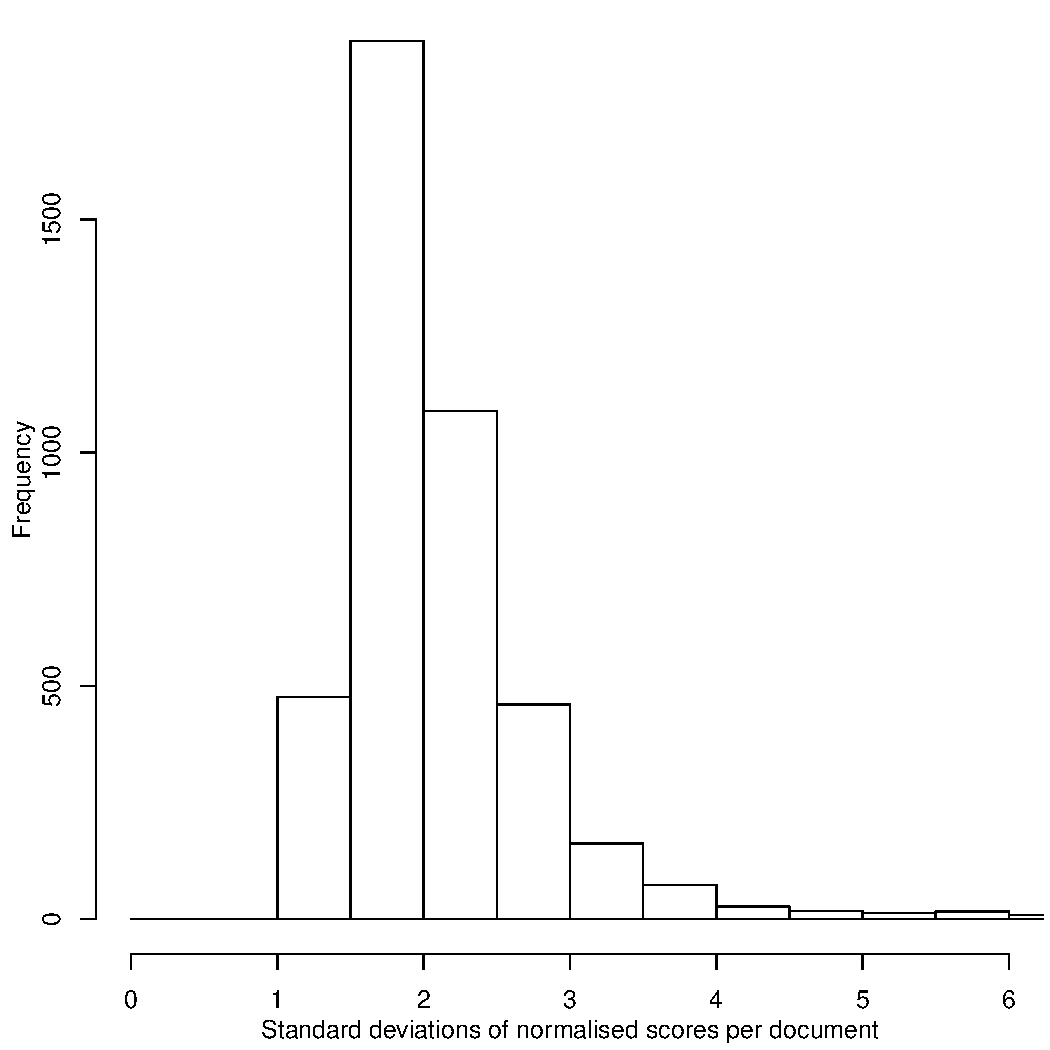
\includegraphics[width=.5\linewidth,page=1]{figs/sample_standard_deviations.pdf}
  \caption{Histogram of standard deviations 
    of the normalized scores for each topic-document in our data.
    There were 53 values greater than 6 which are not shown.
    \label{fig:sampleStandardDeviations}
  }
\end{figure}


\begin{table}[t]
\begin{center}
\tbl{The number of workers required to judge each document 
to be 95\% confident that mean normalized scores are within $E$ of the true population value.
\label{tab-sample-size}
}{%
\begin{tabular}{r rrrrrr}
\hline
     & \multicolumn{6}{c}{$\sigma$} \\ \cline{2-7}
 $E$           &1    & 2  &   3 &    4&     5&     6 \\
\hline
    0.5   & 27  &107 & 239 & 425 & 664  &956 \\
    1.0   &  7  & 27 &  60 & 107 & 166  &239 \\
    1.5   &  3  & 12 &  27 &  48 &  74  &107 \\
    2.0   &  2  &  7 &  15 &  27 &  42  & 60 \\
    2.5   &  2  &  5 &  10 &  17 &  27  & 39 \\
    3.0   &  1  &  3 &   7 &  12 &  19  & 27 \\
    3.5   &  1  &  3 &   5 &   9 &  14  & 20 \\
    4.0   &  1  &  2 &   4 &   7 &  11  & 15 \\
    4.5   &  1  &  2 &   3 &   6 &   9  & 12 \\
    5.0   &  1  &  2 &   3 &   5 &   7  & 10 \\
\hline
\end{tabular}%
}
\end{center}
\end{table}

\textcolor{red}{While this argument is far from being conclusive, it
confirms that the ten workers that we used in our experiment, and the
associated cost, can be reduced.
Therefore, from the about $\$0.4$ for each document figure mentioned in
Section~\ref{sec:crowd-judging} we can estimate that only about $\$0.3$
for each document are really needed, if not less since more efficient
methods could be devised.} 


%%% \aht{not sure where this fits, now}
%%% 
%%% To investigate the robustness of the obtained ME scores, and
%%% correspondingly the necessity of gathering repeat ME judgments, we
%%% calcualte the reliability of the observations using Krippendorff's
%%% $\alpha$. Table~\ref{tab-alpha} shows the $\alpha$ values obtained when 
%%% including the ratings of the first $n=2$ to $10$ ME scores obtained 
%%% for each topic-document pair.
%%% From the results, it can be seen that the ME ratings show remarkably 
%%% consistent levels of agreement, based on the ratio-level $\alpha$
%%% reliability measure.
%%% 
%%% \begin{table}[t]
%%% \begin{center}
%%% \tbl{Agreement between ME
%%% scores assigned by the first $n$ judges, using the ratio difference
%%% function of 
%%% Krippendorff's $\alpha$ reliability measure.
%%% \label{tab-alpha}
%%% }{%
%%% \begin{tabular}{c|cccccccccc}
%%% n & 2 & 3 & 4 & 5 & 6 & 7 & 8 & 9 & 10 \\
%%% \hline
%%% $\alpha$ & 0.327 & 0.321 & 0.322 & 0.322 & 0.317 & 0.321 & 0.320 & 0.322 & 0.323 \\
%%% \end{tabular}%
%%% }
%%% \end{center}
%%% \end{table}

%%%% \sm{ What happens if we chunk the low quality workers? 
%%%%   That would be interesting because we need to disentangle the effect
%%%%   of crowdsourcing (low quality, cheating, etc) and the ME effects
%%%%   (can the scores be reliable? 
%%%%   How? 
%%%%   When?)}
%%%%   \fs{But we (hopefully) got rid of all the low quality workers through
%%%%   our checks. I think it would be useful to do an analysis including
%%%%   fewer repeat judgements instead.}
%%%% 
%%%% \sm{I leave here some notes just not to forget.}
%%%% After some thinking with Eddy, we realized that we can do three
%%%% slightly different things:
%%%% \begin{itemize}
%%%% \item Fewer redundant judgments: What if we collect fewer redundant judgments? (we have 10 in the
%%%%   full data set, what happens with $k<10$?) 
%%%% \item Shorter units: What if we use fewer judgments per worker (or rather unit)? 
%%%%   Our workers expressed 8 judgments each (or, there were 8 judgments
%%%%   per unit). 
%%%%   2 of them are on the \nkn and \hkh docs, so really 6 judgments each.  
%%%%   Let's measure the quality that we get when removing the last
%%%%   document, then the last two, and so on up to keeping just one (we
%%%%   start from the last to avoid learning bias). 
%%%%   In this way we simulate what we would get with workers judging 1-6
%%%%   docs, plus the \nkn and \hkh.
%%%% \item Fewer workers: What if we use fewer workers/unit? 
%%%%   (we have 182--697 units / workers per topic, see
%%%%   Table~\ref{tab:descr-stat}). 
%%%%   We can try randomly removing workers. 
%%%%   This is slightly different from the previous ones... 
%%%%   and we can also think of chunking bad workers on the basis of some
%%%%   quality measure...)
%%%% \end{itemize}
%%%% All these simluations aim at understanding if and how we can, in
%%%% future experiments, \emph{use less data} (and save money!) 
%%%% in some way. 
%%%% We aim at some charts similar to Figure 2 in our ECIR paper.
%%%% 
%%%% Now, quality. 
%%%% We have used Pairwise Agreement (PA) in the rest of the paper; if I
%%%% understood it correctly it should weigh more a disagreement when
%%%% ``there are many other documents in between'', but not the specific ME
%%%% score. 
%%%% We are also attempting to define an agreement measure that takes into
%%%% account the ME scores, not just their order. 
%%%% The basic idea to do that is that any ``mis-swap'' (i.e., any pair of
%%%% documents which is ranked differently in the official judgment (S or
%%%% T) and by the crowd (i.e., considering the median normalized scores)
%%%% is \emph{weighted} by the difference of the median normalized scores. 
%%%% We have thus a Weighted PA (WPA).
%%%% So for example if TREC scores for T(d1)=1 and T(d2)=0, and if
%%%% ME(d1)=10, ME(d2)=11, then this is a disagreement with a lower weight
%%%% than T(d3)=1 and T(d4)=0 ME(d3)=10, ME(d4)=100. 
%%%% PA does not distinguish between the two, WPA does. 
%%%% And of course, once we have a WPA measure, we can use it to re-measure
%%%% agreement also in the rest of the paper.
%%%% 
%%%% Note: we can also use tau on systems besides PA and WPA?
%%%% 
%%%% Note: This WPA considers only the mis-swaps. 
%%%% Can we improve it by weighing also the pairs of documents that are
%%%% ranked in the same order? (It seems not simple to me)
%%%% 
%%%% Note: I've put some papers about agreement measures in the
%%%% Literature folder; have a look! I do not know if there exists a
%%%% measure agreement which is perfect for our purposes (how to define
%%%% agreement between a ratio scale and an ordinal scale, which is not
%%%% even a total rank, seems not easy to me)
%%%% 
%%%% Note: this seems an interesting and not easy piece of work, we might
%%%% consider to add something to this TOIS paper and maybe work on it in
%%%% full detail in another paper (maybe together with the topic difficulty
%%%% issue?) Let's keep this in mind...
%%%% 
%%%% \aht{yes - this interesting. Cannot decide whether to do it here, or in the next paper. For
%%%% ease, it is the next paper :) }
%%%% 


\subsection{Summary}
\label{sec:summary-1}

\textcolor{red}{ 
Using ME with crowdsourcing could potentially raise
several concerns, including: 
subjectiveness of the relevance scale; 
difficulty in normalizing disparate scales from different workers; 
lack of proper training of workers;
potential internal and/or external disagreement between workers;
and high overall cost as redundant workers needed to ensure quality.
On the basis of the results presented so far we can conclude that, at
least with our setting and our quality checks in place (see items
(a)--(d) in Section~\ref{sec:quality-checks}), we can be reassured that
magnitude estimation relevance scores gathered by means of
crowdsourcing are reliable, thus answering RQ\ref{item:rq4}.
Also, the cost to collect the ME judgments in our experiments 
is comparable to that of collecting ordinal scale judgments, 
and there are hints that this cost can be lowered by collecting fewer judgments.
} 

% Local Variables:
% TeX-master: "ME-TOIS.tex"
% End:
